\documentclass[graphics]{beamer}
\usepackage{xcolor}
\usepackage{graphicx}
\usepackage{verbatim}
\usepackage{wrapfig}
\usepackage{tabularx}
\usepackage{multirow}
\usepackage{amssymb}
\usepackage{pifont}
\usepackage{tikz}
\def\Checkmark{\tikz\fill[scale=0.2](0,.35) -- (.25,0) -- (1,.7) -- (.25,.15) -- cycle;} 

\useoutertheme{shadow}
%\usecolortheme{orchid}
\usecolortheme{seahorse}
\newcommand{\cmark}{\text{\ding{51}}}
%\newcommand*{\GtrSim}{\smallrel\gtrsim}

% math commands
\newcommand{\be}{\begin{eqnarray}}
\newcommand{\ee}{\end{eqnarray}}
\newcommand{\beq}{\begin{equation}}
\newcommand{\eeq}{\end{equation}}
\def\simless{\mathbin{\lower 3pt\hbox
      {$\rlap{\raise 5pt\hbox{$\char'074$}}\mathchar"7218$}}}
\def\simgreat{\mathbin{\lower 3pt\hbox
      {$\rlap{\raise 5pt\hbox{$\char'076$}}\mathchar"7218$}}} %> or of order

% variables

\def\toonscale{0.45}
\def\mboxy#1{\mbox{\small #1}}

\defbeamertemplate*{title page}{customized}[1][]
{
  \usebeamerfont{title}\inserttitle\par
  \usebeamerfont{subtitle}\usebeamercolor[fg]{subtitle}\insertsubtitle\par
  \bigskip
  \usebeamerfont{author}\insertauthor\par
  \usebeamerfont{institute}\insertinstitute\par
  \usebeamerfont{date}\insertdate\par
  \usebeamercolor[fg]{titlegraphic}\inserttitlegraphic
}
\begin{comment}
\AtBeginSection[]{
  \frame{
    \frametitle{Outline}
    \tableofcontents[currentsection]
  }
}
\end{comment}


\title{\textcolor{red}{News from the FRB universe}}
%\subtitle{}
\author[U. Pen]{{
{ 
\textcolor{green}{\small CHIME-FRB collaboration, Scintillometry
  collaboration, and more}
}, 
}
\\[8mm] 
\textcolor{blue}{\tiny photo: Andre Renard}
}
\date{\textcolor{red}{January 10, 2019}}


\begin{document}


%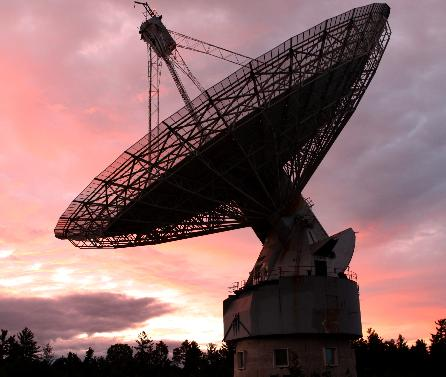
\includegraphics[width=4.4in]{Figures/IMG-7749-ARO-crop.JPG}

\frame{
\vspace{-0.5in}
\begin{center}  
%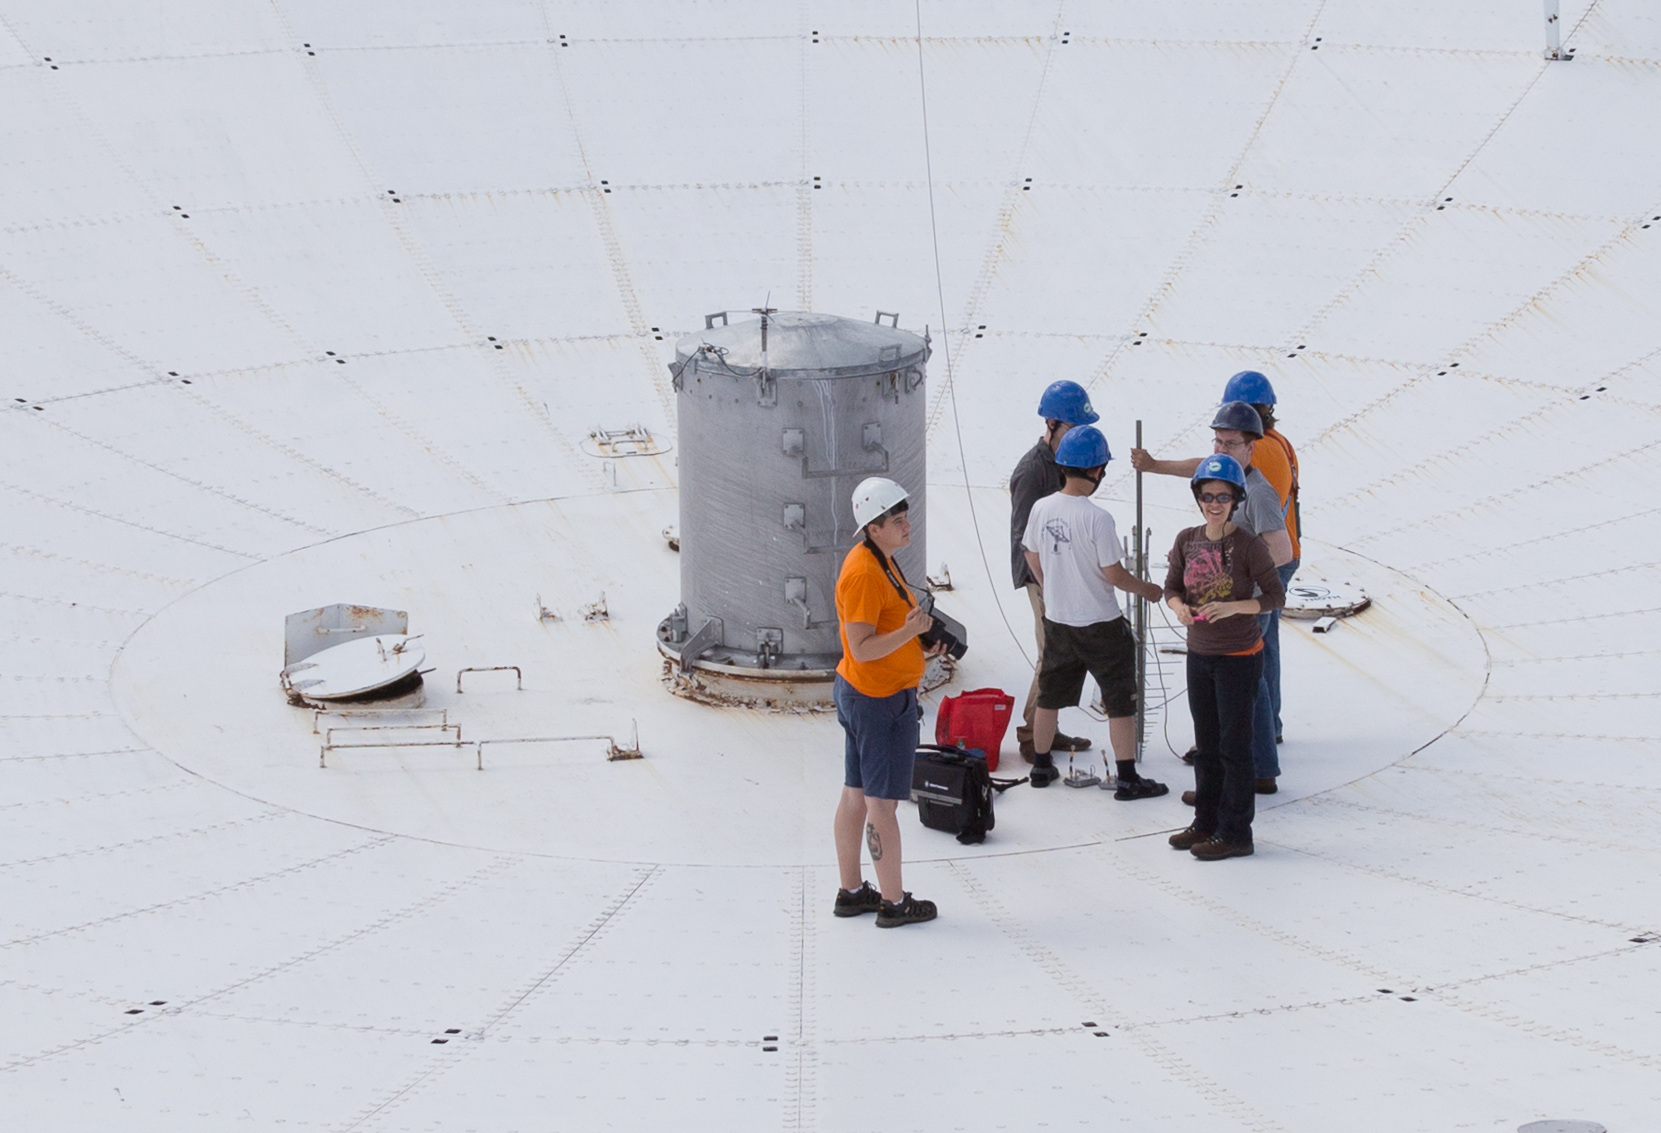
\includegraphics[width=4.4in]{Figures/IMG-0438-by-Andre-cropped.jpg}
\end{center}
\begin{picture}(320,250)
\put(-35,45){
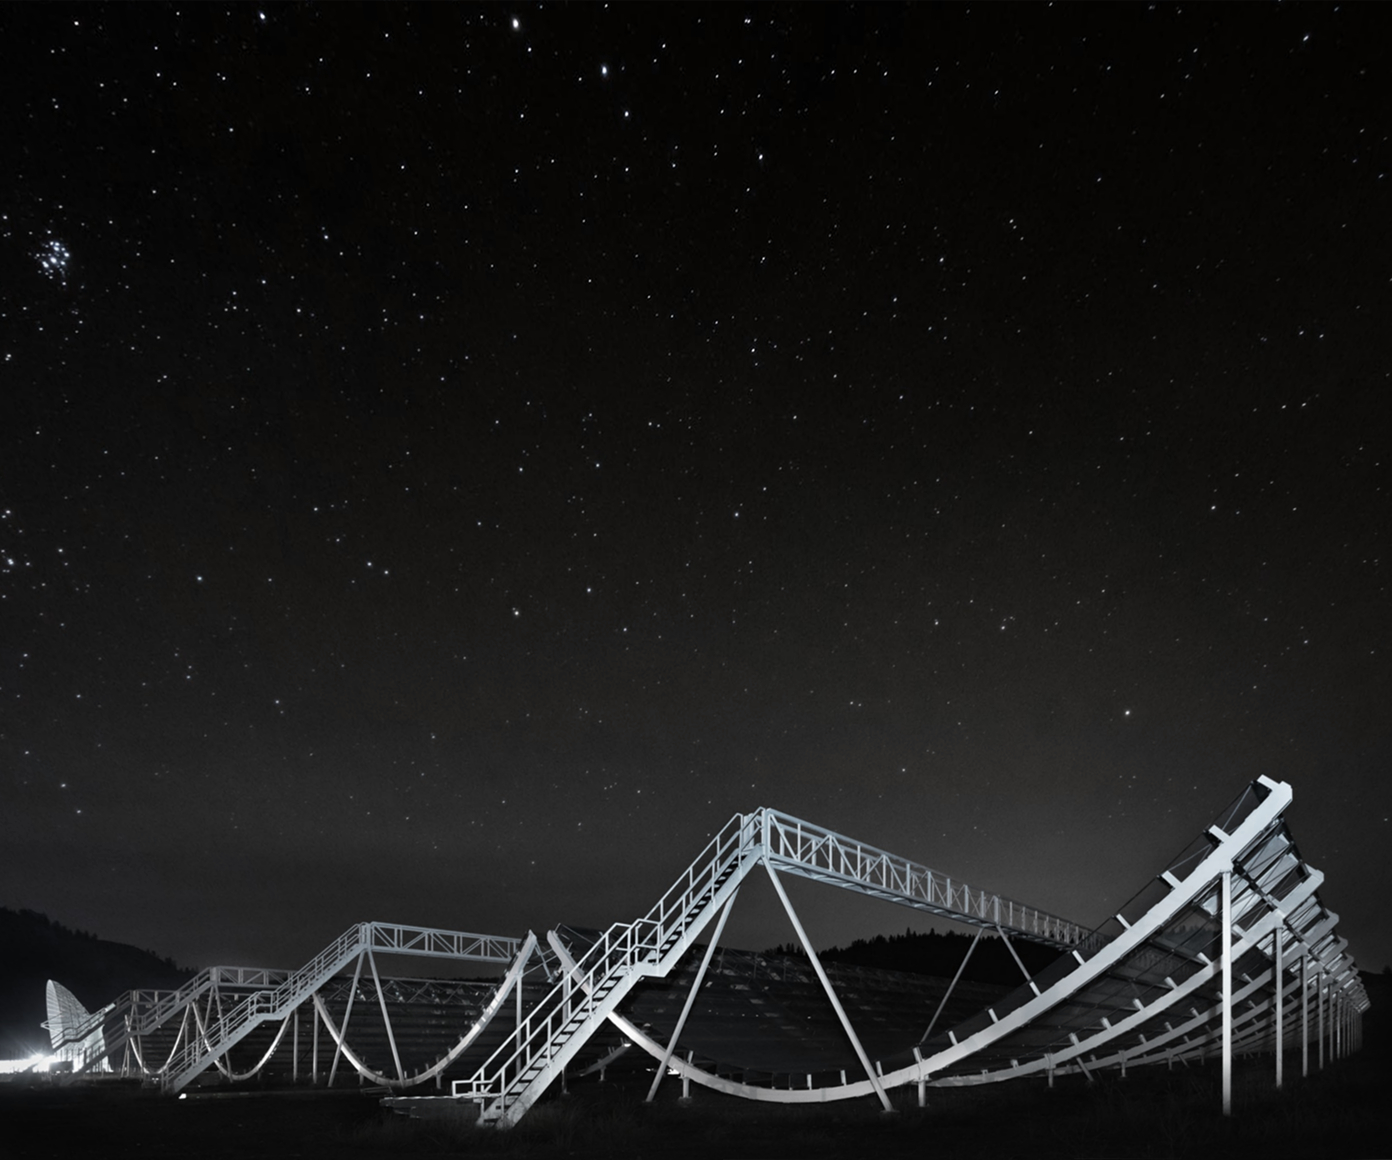
\includegraphics[width=5.1in]{Figures/andre_night_squared_DSC2890.jpg}}
\end{picture}
\vspace{-4in}
\\
image credit: Andre Recnik
\\
\vspace{1in}
\titlepage
}


%\section*{Introduction}
\section{Introduction}

\begin{comment}
  \subsection{Outline}

  \frame{
    \frametitle{Outline}
    \tableofcontents
  }
\end{comment}

  \frame{
    \frametitle{Overview}
    \begin{itemize}
      \item New CHIME results: low frequncy FRB's, repeater
      \item challenges to theory: energetics, coherent emission
      \item what might FRB's be?
      \item what are they good for?
      \item Future prospects
    \end{itemize}
    \vspace{-0.5in}\hspace{2in}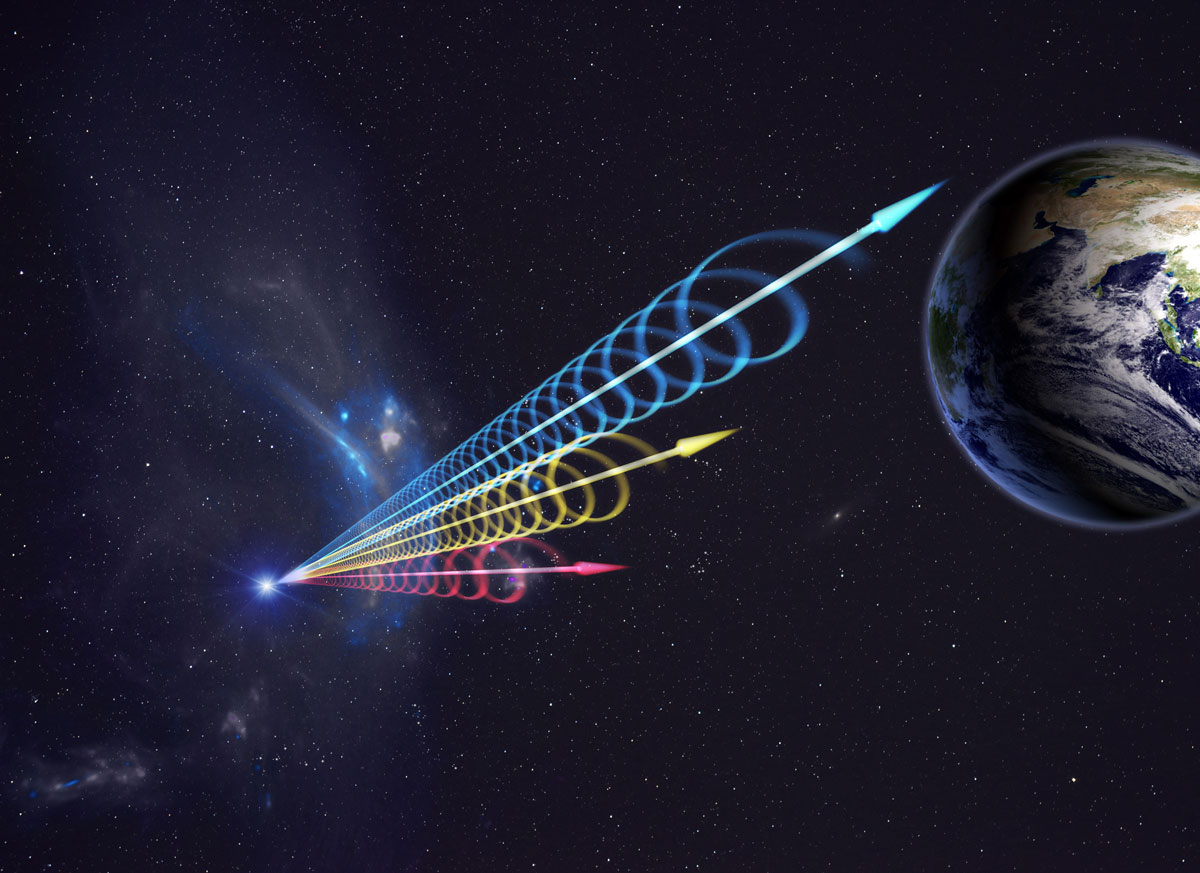
\includegraphics[width=0.6\textwidth]{Figures/imagesnon-gallery2015c-blue12-02-Fast-Radio-BurstsFRB_nrao.jpg}
{\tiny image image credit: Jingchuan Yu, Beijing Planetarium}
  }


  \frame{
    \frametitle{Brief History of FRBs}
    \begin{itemize}
      \item first discovered in 2007, FRB010724
      \item faced with skepticism until 2013 when 4 more were
        confirmed, exhibiting scattering (Thornton et al)
      \item rotation measure and two-screen plasma lensing discovered in 110523 (Masui et al, 2013)
      \item repeater 121102 (Spitler et al 2016)
      \item with high RM ($10^5$)
        \item $\sim$ 50 published          
    \end{itemize}
    \vspace{-0.5in}\hspace{2in}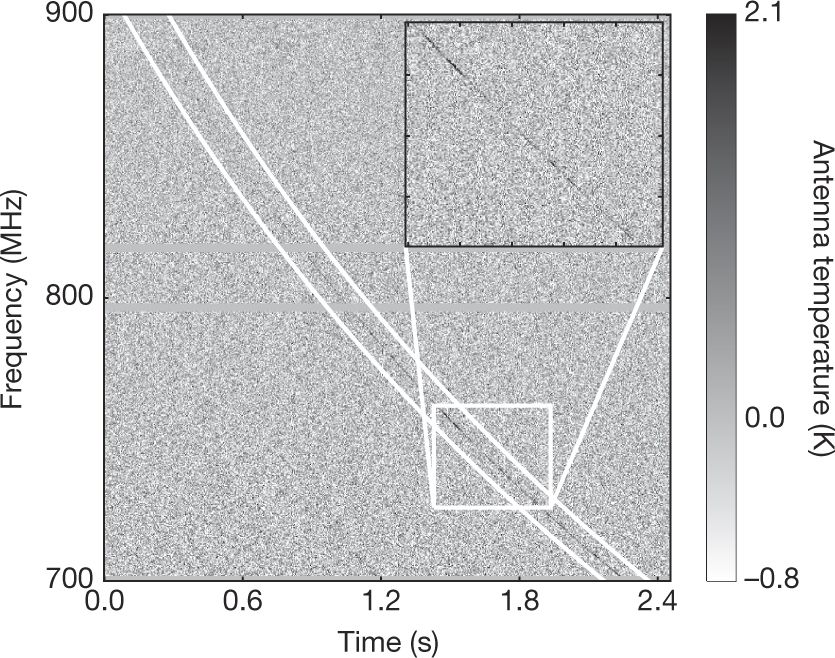
\includegraphics[width=0.6\textwidth]{Figures/nature15769-f1.jpg}
  }


  \frame{
    \frametitle{CHIME-FRB}
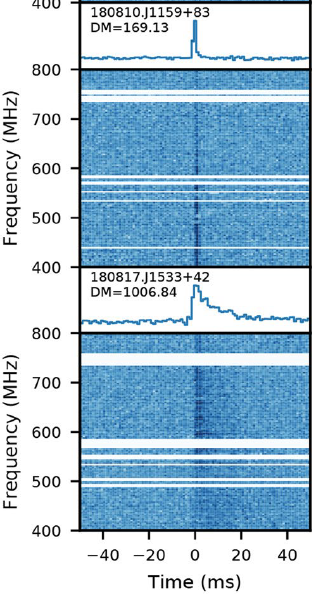
\includegraphics[width=0.35\textwidth]{Figures/chime-frb-precomissioning.png} 
CHIME-FRB collaboration: Nature, Jan 9, 2019
  }

  \frame{
    \frametitle{R2}
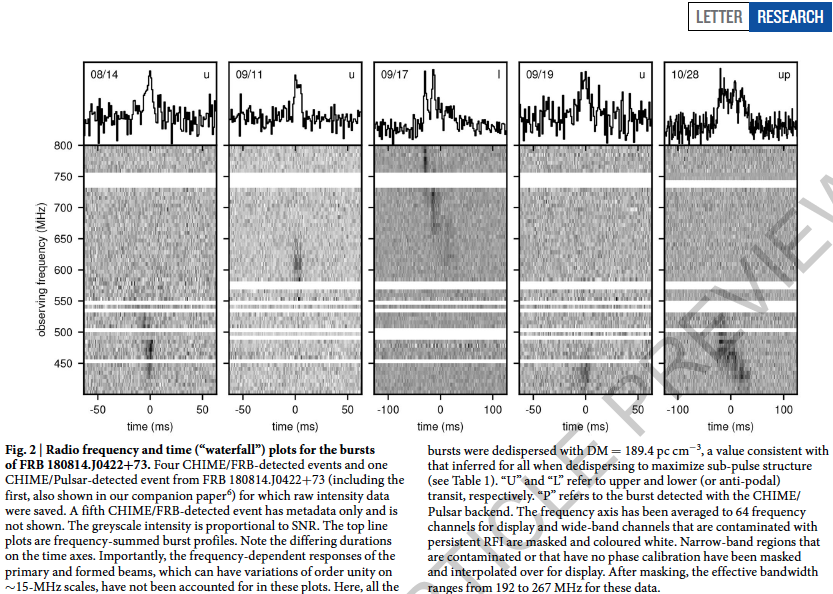
\includegraphics[width=0.9\textwidth]{Figures/chime-R2.png} 
  }

\frame{
    \frametitle{What have we learned?}
    \begin{itemize}
      \item CHIME has unmatched follow-up capability
      \item uncommon repetition is common, perhaps all FRBs repeat
      \item R2 also shows complex narrow frequency-time structure:
        challenge for theory.
      \item many FRB's bright and weakly scattered at bottom of CHIME
        band (400 MHz): excellent probe of plasma propagation effects
      \item 
    \end{itemize}
}




\section{Lensing}

\frame{
    \frametitle{Plasma Lensing}
    \begin{itemize}
      \item galactic scintillation (plasma lensing) provides micro arcsecond probe of
        FRB environment
      \item $\lambda^4$ scattering dependence must be near FRB source:
        not intervener (Vedantham and Phinney 2018)  or IGM
      \item may be source of spectral/temporal structure
    \end{itemize}
}


  \frame{
    \frametitle{Black Widow PSR B1957+20}
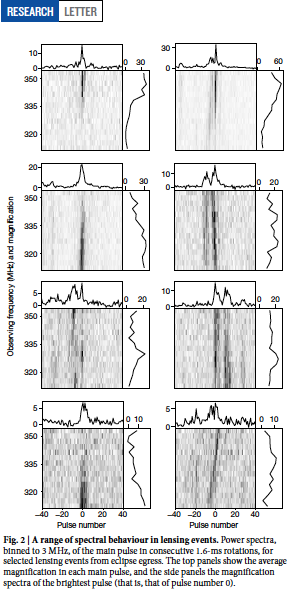
\includegraphics[width=0.35\textwidth]{Figures/black-widow.png}
\vspace{0.5in}
\tiny Main+ 2018
  }

  \frame{
    \frametitle{Applications}
    \begin{itemize}
    \item measure baryon content through cross correlation (McQuinn 2014)
    \item probe extragalactic plasma lensing, magnetic fields
    \item coherent probe of space time, strain $h\sim $ns/Gpc$ \sim 10^{-27}$
    \end{itemize}
  }


  \frame{
    \frametitle{Anomalies}
    \begin{itemize}
    \item ASKAP-Parkes flux tension: are FRB distances host DM dominated?
    \item Is distribution Euclidean?
    \item Are repeaters a different class?
    \item Side lobe detection rate?
    \end{itemize}
  }

  \frame{
    \frametitle{Amusing speculations}
    \begin{itemize}
    \item NS: Magnetar? SLSNe? beamed?
    \item coherent emission outside light cylinder? Crab?
    \item non-magnetar repeaters: Thompson?
    \item black holes?
    \end{itemize}
  }


 \frame{
    \frametitle{Personal speculations}
    \begin{itemize}
    \item nearby, Euclidean, DM dominated by host
    \item special environment: many similarities for J1745-2900 GC magnetar:
    \item high RM, local DM, temporal non-steady RM variation, likely local scattering
    \item possible environments: BH, SNR, PDR      
    \end{itemize}
  }



  \frame{
    \frametitle{Future}
    \begin{itemize}
      \item Observational:
      \item interferometric array localization: ASKAP, VLA, etc
      \item blind VLBI-localization: CHIME-ARO-GBT
      \item more ambitious localizing surveys: CHIME++, SII
      \item Theory:
      \item coherent emission with narrow frequency structure
      \item neutron stars?
      \item Lensing catastrophe theory
      \item testing space-time: gravitational lensing, gravitational
        waves, etc.
    \end{itemize}
  }


  \frame{
    \frametitle{Conclusion}
    \begin{itemize}
      \item CHIME-FRB: new discovery window
      \item FRB challenge: mechanism, uses
      \item must navigate amongst large numbers of wrong papers
    \end{itemize}
  }

\end{document}
